\mode<presentation>
{
% Use default, for more space!
%  \usetheme{Warsaw}
}

%\usepackage[english]{babel}
\usepackage[utf8]{inputenc}

% Note: using version 2.0-alpha3
\usepackage[cache]{minted}

% Hour-long talk

\title{Exploring type-directed, test-driven development}
\subtitle{A case study using FizzBuzz}
\author{Franklin Chen}
\institute{http://franklinchen.com/}
\date[Pittsburgh TechFest 2014]{June 7, 2014 \\ \href{http://www.pghtechfest.com/}{Pittsburgh TechFest 2014}}

\subject{Talks}

% Delete this, if you do not want the table of contents to pop up at
% the beginning of each subsection:
%\AtBeginSubsection[]
%{
%  \begin{frame}<beamer>{Outline}
%    \tableofcontents[currentsection,currentsubsection]
%  \end{frame}
%}

\begin{document}

\maketitle

\begin{abstract}
  An expressive static type system is one of the most joyful and
  powerful tools for prototyping, designing, and maintaining
  programs. In this performance-theatrical presentation, I will
  provide a taste of how to use types, in conjunction with tests, to
  drive iterative development of a particular program, the famous
  FizzBuzz problem. We will solve generalizations of this problem,
  changing and adding requirements, to illustrate the pleasures and
  benefits of ``type thinking''.

  The Scala language will be used as the vehicle for this
  demonstration, but the techniques apply immediately to any
  industrial-strength statically typed language, such as Haskell,
  OCaml, F\#, Rust, and most recently, Swift.

  (Note: this presentation will use live human volunteers to play the
  roles of various programming concepts.)
\end{abstract}

\begin{frame}
  \titlepage
\end{frame}

\section*{Outline}

\begin{frame}{Outline}
  \begin{itemize}
  \item Introduction
  \item Original \texttt{FizzBuzz}
  \item \texttt{FizzBuzz} 2
  \item \texttt{FizzBuzz} 3
  \item Parallel \texttt{FizzBuzz}
  \item Conclusion
  \end{itemize}
%  \tableofcontents
%  \tableofcontents[pausesections]
\end{frame}

% Since this a solution template for a generic talk, very little can
% be said about how it should be structured. However, the talk length
% of between 15min and 45min and the theme suggest that you stick to
% the following rules:  

% - Exactly two or three sections (other than the summary).
% - At *most* three subsections per section.
% - Talk about 30s to 2min per frame. So there should be between about
%   15 and 30 frames, all told.

\section{Introduction}

\subsection{Goals}

\begin{frame}{Goals of this presentation}
  \begin{itemize}
  \item Give a taste of a \alert{type}-directed, \alert{test}-driven software development process.
    \begin{itemize}
    \item See testing frameworks in action.
    \item See types in action.
    \end{itemize}
  \item Using \texttt{FizzBuzz} because:
    \begin{itemize}
    \item The basic problem is easy to understand.
    \item Modifications will be easy to understand.
    \item You will see something surprising and cool!
    \end{itemize}
  \item Encourage you to explore further.
  \end{itemize}
\end{frame}

\subsection{Test-driven development (TDD)}

\begin{frame}{What is test-driven development (TDD)?}
  \begin{itemize}
  \item First, write a test case.
  \item Then, write code.
  \item Rerun the test.
  \item Repeat.
  \end{itemize}
\end{frame}

\subsection{Type systems}

\begin{frame}{What is a type system?}
  \begin{itemize}
  \item For this presentation: a \alert{syntactic} method for \alert{proving} the absence of certain program behaviors.
  \item Versus: runtime tag system.
  \end{itemize}

  ``Debating'' types ``versus'' tests?
  \begin{itemize}
  \item Let's not argue.
  \item Let's use both!
  \end{itemize}
\end{frame}

\subsection{Crappy versus decent type systems}

% Last-minute inclusion of Rust and Swift!
\begin{frame}{Crappy versus decent type systems}
  \begin{itemize}
  \item Archaic \alert{1960s-1970s}-era type systems give types a bad reputation!
    \begin{itemize}
    \item C, C++, Objective C
    \item Java
    \end{itemize}
  \item ``Modern'' \alert{1980s-1990s}-era type systems.
    \begin{itemize}
    \item ML (\href{http://www.smlnj.org/}{Standard ML}, \href{http://ocaml.org/}{OCaml}, \href{http://fsharp.org/}{F\#}): I first used in 1994 (20 years ago)
    \item \href{http://www.haskell.org/}{Haskell}: I first used in 1995
    \item \href{http://www.scala-lang.org/}{Scala}: first released in 2004
    \item \href{http://www.rust-lang.org/}{Rust}: not yet version 1.0
    \item \href{http://developer.apple.com/swift/}{Swift}: announced by Apple on June 2, 2014!
    \end{itemize}
  \end{itemize}
\end{frame}

\section{The original FizzBuzz problem}

\subsection{Original FizzBuzz problem statement}

\begin{frame}{Original FizzBuzz problem statement}
  \begin{quotation}
Write a program that prints the numbers from 1 to 100. But for multiples of three, print ``Fizz'' instead of the number. And for the multiples of five, print ``Buzz''. For numbers which are multiples of both three and five, print ``FizzBuzz''.
  \end{quotation}
\end{frame}

\subsection{Starter Scala code: main driver}

\begin{frame}[fragile]{Starter Scala code: main driver}
  \begin{center}
    
\includegraphics[height=1cm]{scala-logo-red-dark.png}
  \end{center}

  Let's use Scala, a modern \alert{object-oriented} and \alert{functional} language.

  \inputminted{scala}{Main1.scala}

  \begin{itemize}
  \item Type-directed design: separate out effects (such as printing to terminal) from the real work.
  \item Type-directed feedback: compilation fails when something is not implemented yet.
  \end{itemize}
\end{frame}

\subsection{The joys of continuous compilation and testing}

\begin{frame}[fragile]{The joys of continuous compilation and testing}
  \begin{center}
    
\includegraphics[height=0.75cm]{sbt-logo-orange-600x360.png}
  \end{center}

  Let's use \href{http://www.scala-sbt.org/}{SBT}, a build tool supporting Scala, Java, etc.

  \begin{itemize}
  \item \href{http://www.scala-sbt.org/release/docs/Detailed-Topics/Triggered-Execution.html}{Source file changes trigger smart recompilation!}
  \item Source file changes trigger rerun of the tests that depend on changed code!
  \end{itemize}

  \inputminted{console}{testQuick.console}
\end{frame}

\begin{frame}[fragile]{Fix compilation error using stub}
  \inputminted{scala}{Main2.scala}

  \begin{itemize}
  \item Write desired type signature.
  \item \mintinline{scala}{???} is super-convenient for stubbing.
    \begin{itemize}
    \item From Scala standard library.
    \item Just does \mintinline{scala}{throw new NotImplementedError}.
    \end{itemize}
  \end{itemize}
\end{frame}

\subsection{Acceptance test (simplified)}

\begin{frame}[fragile]{Acceptance test (simplified)}
  \begin{center}
    
\includegraphics[height=0.75cm]{specs2.png}
  \end{center}

  Let's use \href{http://specs2.org/}{specs2}, a popular testing framework for Scala, Java, etc.

  \inputminted{scala}{MainSpec1.scala}

  \begin{itemize}
  \item A realistic acceptance test would involve I/O.
  \item Omitted in presentation to save time.
  \end{itemize}
\end{frame}

\begin{frame}[fragile]{The test compiles, but fails}
  
  \begin{itemize}
  \item Save brand new source file \texttt{MainSpec.scala}.
  \item Incremental compilation/testing continues.
  \end{itemize}

  \inputminted{console}{testQuick2.console}
\end{frame}

\begin{frame}[fragile]{Outside-in: toward a \mintinline{scala}{FizzBuzz} unit}
  Use types to assemble code like shapes in a jigsaw puzzle:

  \inputminted{scala}{Main4.scala}

  \begin{center}
    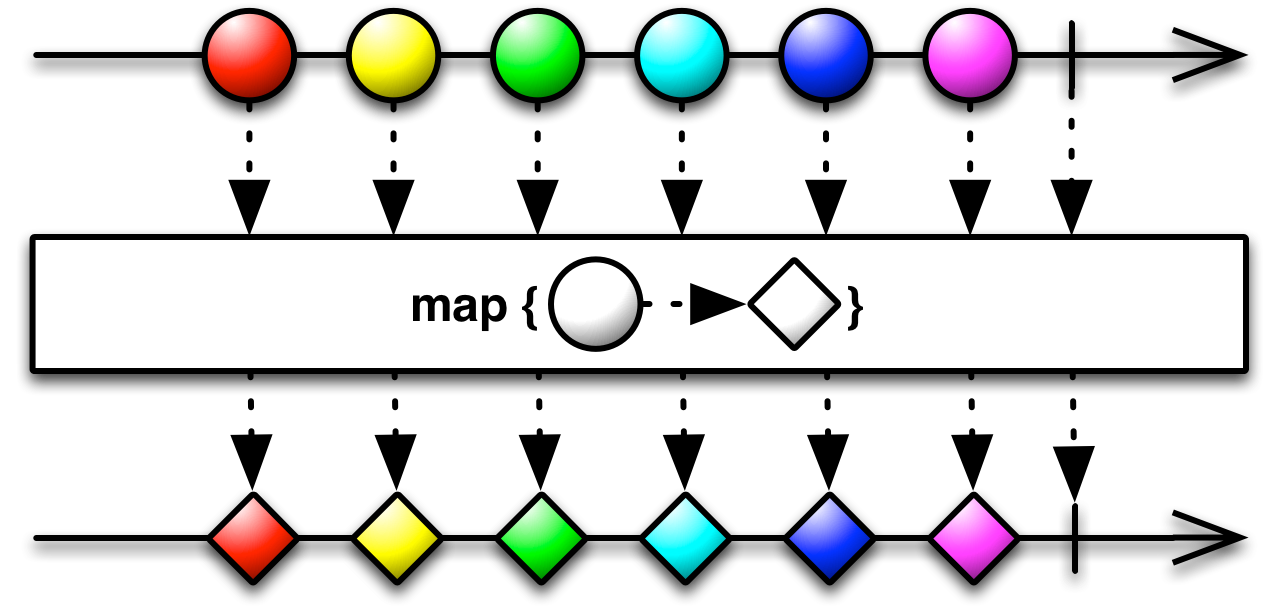
\includegraphics[height=2.5cm]{map.png}
  \end{center}

  \begin{itemize}
  \item \mintinline{scala}{(start to end): Seq[Int]}, where \href{http://www.scala-lang.org/api/2.11.0/index.html\#scala.collection.Seq}{\mintinline{scala}{Seq[_]}} is a \alert{type constructor} that, given a type \mintinline{scala}{A}, returns a type of \mintinline{scala}{Seq[A]}.
  \item For any value of type \mintinline{scala}{Seq[A]}, \mintinline{scala}{map: (A => B) => Seq[B]}.
  \item So, we need to implement \mintinline{scala}{FizzBuzz.evaluate: Int => String}.
  \end{itemize}
\end{frame}

\subsection{Test-driven units}

\begin{frame}[fragile]{Starting the \texttt{FizzBuzz} module}
  \inputminted{scala}{FizzBuzz1.scala}

  \begin{itemize}
  \item Acceptance test drives need for units.
  \item Outside-in implementation drives discovery of a type:      
    \mintinline{scala}{Int => String}.
  \item I like to write \alert{type synonyms} as \alert{documentation}:
    \begin{itemize}
    \item \mintinline{scala}{type FizzBuzzer = Int => String}.
    \item I dislike \alert{comments}. Comments are not executable and checkable, unlike types and tests.
    \end{itemize}
  \end{itemize}
\end{frame}

\begin{frame}[fragile]{First unit tests: example-based}
  \inputminted{scala}{FizzBuzzSpec1.scala}
\end{frame}

\subsection{Property-based tests}

\begin{frame}[fragile]{The joy of property-based tests}
  \begin{center}
    
\includegraphics[height=0.75cm]{logo_forall_h61.png}
    
\includegraphics[height=0.75cm]{logo_scalacheck_h61.png}
  \end{center}

  Let's use \href{http://scalacheck.org/}{ScalaCheck} to write \alert{property-based} tests.

  \inputminted{scala}{FizzBuzzSpec2.scala}

  \begin{itemize}
  \item \alert{Type-driven}: here, random \mintinline{scala}{Int} values are generated.
  \item Automatically randomly generates tests for each property (defaults to 100).
  \end{itemize}
\end{frame}

\begin{frame}[fragile]{Property-based tests, continued}
  The other three cases of interest:

  \inputminted{scala}{FizzBuzzSpec3.scala}
\end{frame}

\subsection{Solving the FizzBuzz problem}

\begin{frame}[fragile]{A wrong and ugly solution}
  \inputminted[gobble=2]{scala}{FizzBuzzIf.scala}

  \inputminted{console}{testQuick3.console}
\end{frame}

\begin{frame}{Booleans are evil!}
  The \href{http://en.wikiquote.org/wiki/Colossal\_Cave\_Adventure}{``maze of twisty little conditionals, all different''}.

  \begin{itemize}
  \item Conditions can be arbitrary: depend on \alert{any} combination of data.
  \item A computation leading to a Boolean value by essence \href{http://existentialtype.wordpress.com/2011/03/15/boolean-blindness/}{loses information about the original data}.
  \item Multiple conditions: combinatorial explosion (two conditions led to four cases).
  \item Possibly overlapping conditions: order dependency subtleties.
  \item Possibly duplicated checking of the some condition.
  \item \textbf{No help from type system to catch wrongly written sets of nested, combined conditionals}.
  \end{itemize}

\end{frame}

\begin{frame}[fragile]{Pattern matching organizes information}
  \inputminted[gobble=2]{scala}{FizzBuzz2.scala}

  \begin{itemize}
  \item Visual \alert{beauty} and clarity.
  \item No ordering dependency.
  \item No overlapping.
  \item No duplicated conditionals.
  \item \alert{Type checker} verifies \alert{full coverage} of cases.
  \end{itemize}
\end{frame}

\begin{frame}[fragile]{Example of non-exhaustive pattern matching}
  \inputminted[gobble=2]{scala}{FizzBuzz2Bad.scala}

  \inputminted{console}{testQuick4.console}
\end{frame}

\begin{frame}[fragile]{Acceptance test passed, finally}

  \inputminted{console}{testQuick5.console}

  Are we done?
\end{frame}

\section{FizzBuzz 2: allow configuration}

\subsection{Adding new features}

\begin{frame}{Adding new features}
  Client was pleased with our \texttt{FizzBuzz} solution.

  In the real world, we are never ``done''. Client wants to:
  \begin{itemize}
  \item Specify two \alert{arbitrary} divisors in place of \mintinline{scala}{3} and \mintinline{scala}{5} (such as \mintinline{scala}{4} and \mintinline{scala}{7}).
  \item Specify other \alert{arbitrary} words in place of \mintinline{scala}{"Fizz"} and \mintinline{scala}{"Buzz"} (such as \mintinline{scala}{"Moo"} and \mintinline{scala}{"Quack"}).
  \end{itemize}
\end{frame}

\subsection{Type-driven refactoring}

\begin{frame}{Type-driven refactoring}
  Types make refactoring much more fun.

  \begin{itemize}
  \item Add \alert{new} tests.
  \item Change types and code enough to make the new tests \alert{type check}.
  \item \alert{Refactor} the original code to use the new APIs.
  \item Keep passing the \alert{old} tests.
  \end{itemize}
\end{frame}

\begin{frame}[fragile]{More features means more types}
  Change \mintinline{scala}{Main.runToSeq} driver:
  \inputminted[gobble=2]{scala}{Main5.scala}

  Add new types to \mintinline{scala}{FizzBuzz} module:
  \inputminted[gobble=2]{scala}{FizzBuzz3.scala}
\end{frame}

\begin{frame}[fragile]{Extract original default configuration}
  \inputminted{scala}{Defaults1.scala}
\end{frame}

\begin{frame}[fragile]{More types means more tests}
  A property-based test over \alert{arbitrary} user configurations:
  \inputminted[gobble=2]{scala}{FizzBuzzSpec6.scala}
\end{frame}

\subsection{Refining types}

\begin{frame}[fragile]{Our config type was too coarse}
  \inputminted{console}{testQuick6.console}

  \begin{itemize}
  \item \mintinline{scala}{0} as a divisor \alert{crashes}!
  \item Discovery of client's \alert{underspecification}.
  \item We talk to client: client meant only divisors within \mintinline{scala}{2} and \mintinline{scala}{100}.
  \end{itemize}

  Need to:
  \begin{itemize}
  \item Incorporate runtime \alert{validation} when constructing \mintinline{scala}{Config}.
  \item Correct our random \mintinline{scala}{Config} generator.
  \end{itemize}
\end{frame}

\begin{frame}[fragile]{Add runtime validation}
  (Quick and dirty) \alert{runtime} precondition checking using Scala standard library throwing an \alert{exception} (\href{http://blog.jessitron.com/2013/06/whats-dirtier-than-comments-exceptions.html}{yuck}).

  \inputminted[gobble=2]{scala}{FizzBuzz3Validate.scala}
\end{frame}

\begin{frame}[fragile]{More notes on validation}
  \begin{itemize}
  \item (No time to cover): in real life, prefer type-based solution such as \href{http://eed3si9n.com/learning-scalaz/Validation.html}{Scalaz validation}.
  \item Note: there are languages with more powerful type systems (\href{http://en.wikipedia.org/wiki/Dependent_type}{dependent type system}), such as \href{http://www.idris-lang.org/}{Idris}, that enable defining and checking more precise types (such as ``integer within 2 and 100'').
    \begin{itemize}
    \item \href{http://heartbleed.com/}{Heartbleed} could have been \href{http://bluishcoder.co.nz/2014/04/11/preventing-heartbleed-bugs-with-safe-languages.html}{prevented by coding in the systems language ATS}.
    \end{itemize}
  \item Do not use a weaker type system as an \alert{excuse} not to write tedious validation code or tests!
    \begin{itemize}
    \item Heartbleed could have been prevented using \href{http://martinfowler.com/articles/testing-culture.html}{good validation and testing practices}.
    \end{itemize}
  \end{itemize}
\end{frame}

\begin{frame}[fragile]{Improve random config generator}
  \inputminted[gobble=2]{scala}{FizzBuzzSpec7.scala}
\end{frame}

\begin{frame}[fragile]{New test runs further, stills fails}
  Now refactor old code to \mintinline{scala}{FizzBuzz.compile}:

  \inputminted{scala}{FizzBuzz3Compile.scala}

  \begin{itemize}
  \item Old tests now succeed.
  \item New test also succeeds.
  \end{itemize}
\end{frame}

\section{FizzBuzz 3: \texttt{FizzBuzzPop}}

\subsection{Generalizing to more than two divisors}

\begin{frame}[fragile]{Generalizing to more than two divisors}
  Our client wants us to support \texttt{FizzBuzzPop}:
  \begin{itemize}
  \item Specify three divisors, such as 3, 5, 7.
  \item Print a string combining segments of three words, such as \mintinline{scala}{"Fizz"}, \mintinline{scala}{"Buzz"}, \mintinline{scala}{"Pop"}; or a numerical string if an integer is not a multiple of any of 3, 5, 7.
  \item Still get to choose the three words.
  \item Example: \mintinline{scala}{21} should output \mintinline{scala}{"FizzPop"}.
  \end{itemize}

  How to refactor to support \texttt{FizzBuzzPop}?
\end{frame}

\begin{frame}{Thought-driven development}
    Software development is not primarily about \alert{coding}, but \alert{thinking}.

  \begin{itemize}
  \item Deep fact: solving a more general problem is often easier than solving the specific problem.
  \item There are four important numbers in the Universe:
    \begin{description}
    \item[0] emptiness
    \item[1] existence
    \item[2] other (relationship)
    \item[many] community
    \end{description}
  \end{itemize}
\end{frame}

\subsection{More features means more types (again)}

\begin{frame}[fragile]{More features means more types (again)}
  Write new tests for a proposed \mintinline{scala}{Defaults.fizzBuzzPopper}:

  \inputminted[gobble=2]{scala}{FizzBuzzSpec5.scala}

  Add \mintinline{scala}{Defaults.fizzBuzzPopper}:
  \inputminted[gobble=2]{scala}{Defaults2.scala}
\end{frame}

\begin{frame}[fragile]{Test-driven type refactoring (again)}
  \inputminted{console}{testQuick8.console}

  Change \alert{type} \mintinline{scala}{Config} to allow a sequence of pairs rather than just two:

  \inputminted[gobble=2]{scala}{FizzBuzz3Seq.scala}

  Note how our iterative development process promotes \alert{reuse} (here, of validation logic).
\end{frame}

\begin{frame}[fragile]{Fix remaining type errors}
  Most significant required change reveals the unimplemented case of more than two divisors:
  \inputminted[gobble=2]{scala}{FizzBuzz3SeqCompile.scala}
\end{frame}

\begin{frame}[fragile]{General observations}
  \begin{itemize}
  \item Return a sum of a subset of the configured words, if there is any divisor match.
  \item If there is \alert{no} divisor match, return the numerical string.
  \end{itemize}
\end{frame}

\begin{frame}[fragile]{More computation equals more types}
  \begin{itemize}
  \item Each potential divisor (such as 3, 5, or 7 in \texttt{FizzBuzzPop}) should result in a \alert{rule} that can be applied to any input number to get a string.
  \item Once we have a bunch of rules, we can apply them all to the input, then combine the partial results.
  \end{itemize}

  \inputminted[gobble=2]{scala}{FizzBuzz4.scala}
\end{frame}

\subsection{Demo}

\begin{frame}{Demo time}
  Demo time!

  Volunteers, please step up to demonstrate \texttt{FizzBuzzPop}!
\end{frame}

\begin{frame}[fragile]{Jigsaw puzzle time again}
  \inputminted[gobble=2]{scala}{FizzBuzz5.scala}
\end{frame}

\begin{frame}[fragile]{Test failure reflecting poor use of types}
  Did you see this coming?

  \inputminted[gobble=2]{console}{testQuick9.console}

  Property-based testing again shows us the \alert{unexpected}.

  \begin{itemize}
  \item Empty ``fizz'' and ``buzz'' words are a strange corner case.
  \item Unexpected ambiguity:
    \begin{description}
    \item[Intended behavior] Output a number only if it has none of the divisors.
    \item[Actual behavior] 1649349 is divisible by 13 but not 91, yet 1649349 was output.
    \end{description}
  \end{itemize}

  Why?
\end{frame}

\subsection{\mintinline{scala}{Option[A]} type}

\begin{frame}{An empty string is \alert{not} equivalent to no string}
  Presence of something ``empty'' is \alert{not} equivalent to the absence of something (contrary to how some programming languages work).

  \begin{description}
  \item[Problem] Special case condition, testing for an empty string, conflated an empty combined string with ``failed to be a multiple at all''.
  \item[Solution] Add another type!
  \end{description}
\end{frame}

\begin{frame}[fragile]{\mintinline{scala}{Option[A]} type}

  \mintinline{scala}{Option[A]} is one of two possibilities:
  \begin{itemize}
  \item \mintinline{scala}{None}
  \item \mintinline{scala}{Some(a)} wraps a value \mintinline{scala}{a} of type \mintinline{scala}{A}.
  \end{itemize}

  For example, \mintinline{scala}{Some("")} is not the same as \mintinline{scala}{None}:
  \inputminted{scala}{OptionExample1.scala}
\end{frame}

\begin{frame}[fragile]{Cleaning up the types}
  Change type \mintinline{scala}{Rule}:
  \inputminted[gobble=2]{scala}{FizzBuzz6.scala}

  Immediately get type errors:

  \inputminted[gobble=2]{console}{testQuick10.console}
\end{frame}

\begin{frame}[fragile]{Fix the type errors}

  \inputminted[gobble=2]{scala}{FizzBuzz7.scala}
\end{frame}

\begin{frame}[fragile]{Monoids}
  ``Addition'' for \mintinline{scala}{Option[String]}:
  \inputminted[gobble=2]{scala}{FizzBuzz8.scala}
  
  \href{http://en.wikipedia.org/wiki/Monoid}{Monoid}:
  \begin{itemize}
  \item There is an identity element.
  \item There is a binary associative operator.
  \end{itemize}
\end{frame}

\section{Parallel \texttt{FizzBuzz}}

\begin{frame}[fragile]{Parallelism}
  \begin{itemize}
  \item All code here using \alert{map} can be parallelized; Scala provides high-performance \href{http://scala-blitz.github.io/}{parallel collections}.
  \item The place where \alert{reduce} is used can be parallelized because of the monoid property.
  \item We discovered a theoretical speedup for generalized \texttt{FizzBuzz} from $O(n)$ to $O(\log n)$ (subtleties omitted).
  \end{itemize}
\end{frame}

\begin{frame}[fragile]{Parallelism (code)}
  \inputminted[gobble=2]{scala}{FizzBuzz9.scala}
\end{frame}

\section*{Conclusion}

\begin{frame}{Conclusion}
  \begin{itemize}
  \item \alert{Tests} are useful.
  \item \alert{Types} are useful.
  \item Tests and types work well together to drive design and program evolution!
  \end{itemize}

  All materials for this talk are available at \url{https://github.com/franklinchen/talk-on-type-directed-tdd-using-fizzbuzz}. The hyperlinks on the slide PDFs are clickable.
\end{frame}

%\appendix


\end{document}

%%% Local Variables: 
%%% mode: latex
%%% TeX-master: "presentation"
%%% End: 
